\chapter{Introduction}
The Simulation Soccer 2D League of \cite{robocup} (Sim2d) is one of the most matures leagues of the competition having started in 1996. One of the tasks of the intelligent agents is the defense line. It consists of knowing the timing to intercept the ball or do a clever mark (blocking future shoots or passes). A bad timing will lead to an attacker's dribble or pass and probably a goal. Supervised Learning and deterministic algorithms are the usual techniques used by the TOP 5 teams to solve that problem. Recent researches using Deep Reinforcement Learning to train autonomous agents in multi-agent systems have shown that it outperforms agents based on supervised or deterministic algorithms. The team CYRUS2019, \cite{cyrus}, has released defensive players trained with Deep Reinforcement Learning achieving in third place on RoboCup2019. This work compares three DRL techniques for defensive agents based on CYRUS2019 adapting the Half Field Offensive environment to an OpenAI GYM, \cite{gym}, like environment and apply the best technique on \cite{robocin} agents.

With the goal of beating the human soccer World Champion team in 2050, Robocup has been a great competition to develop and share robotics and autonomous agents techniques. Among the leagues, Soccer Simulation 2D league is a great domain to invest machine learning (ML) algorithms and it is been a challenge as \cite{RoboCupAIChallenge} say. At the very beginning of the league at 1996, the competitors used to implement by their own hands the behaviours of the players. Once it's a simulated league, Machine Learning techniques became natural since there is no mechanic or electronic interference. The German team, Brainstormers was one of the pilots with an approach using Reinforcement Learning (\cite{brainstormers2002}). Since then teams frequently uses Artificial Intelligence algorithms to have unnatural and unpredictable behaviours. 

\begin{figure}[H]
    \centering
    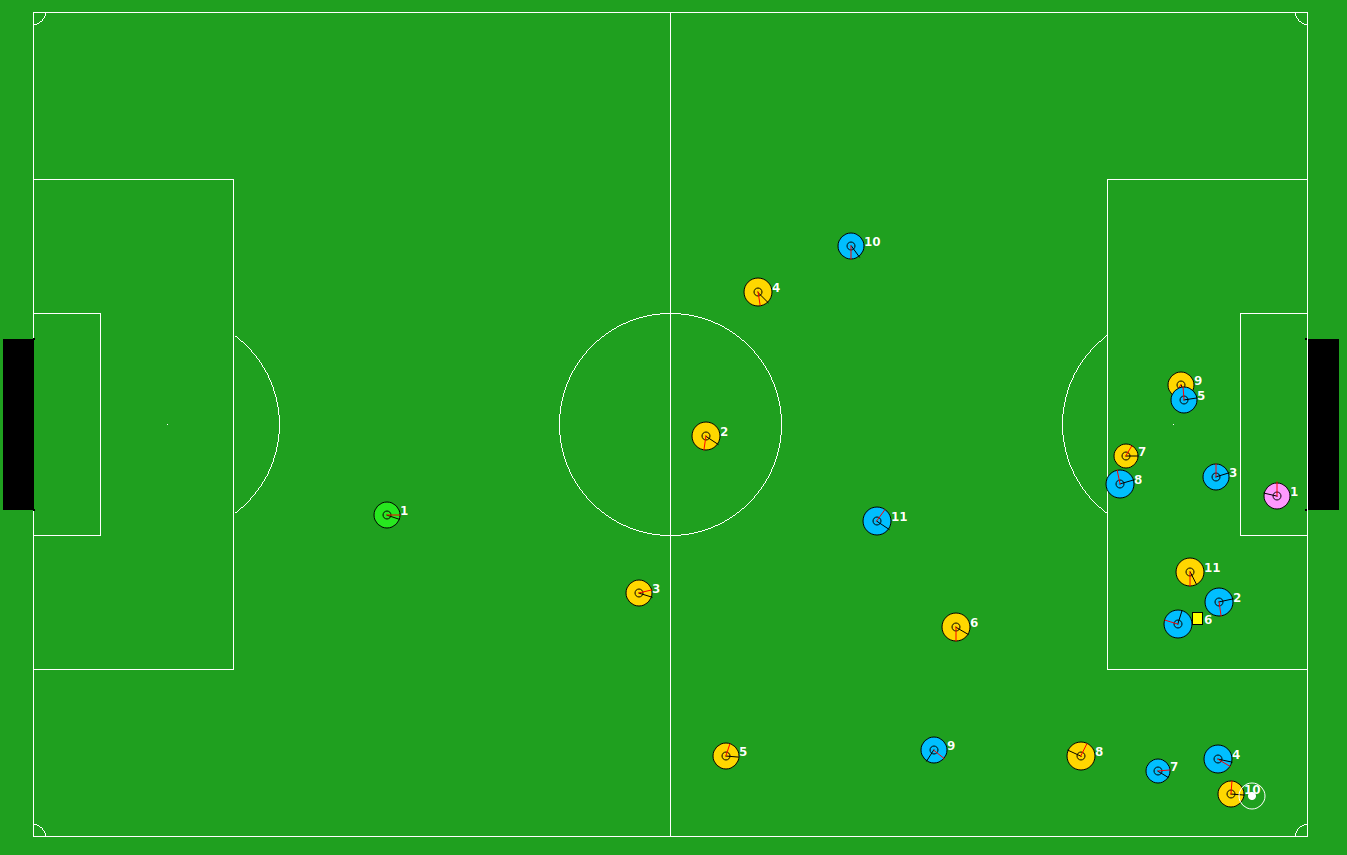
\includegraphics[scale=0.2]{images/ss2dex.png}
    \caption{Example of real game of Simulation Soccer 2D League.}
    \label{fig:ss2dex}
\end{figure}

This work focus on the defense line, specifically in a single intelligent defender cooperating with a hand-coded goalie against a single attacker. As there is more works about the attackers like \cite{passingCrit}, \cite{keepawayRL} and more recent \cite{hausknecht2015deep}, the defense line became attractive to the RoboCIn team.

\cite{deepmind} researchers \cite{dqn} have shown that Deep Q Learning was so effective on Atari games that it outplays human controlled agents. In 2015 Deepmind's AlphaGo agent, \cite{alphago}, won from the European Go Champion Fan Hui and later on 2016 from Lee Sedol, one of the best worldwide. Since then OpenAI and DeepMind has invested a lot of effort on Reinforcement Learning (RL) and Autonomous Agents (AA) systems. Recently \cite{openai5} has become the best agent on \cite{dota2} on 1v1 games and it has a great teamwork performance on 5v5 games winning from most of amateur teams and a few professionals.

Inspired by those recent researches \cite{cyrus} modeled a defensive autonomous agent and it has almost the same efficiency of the champions' Fractals (\cite{glidersv2}, and Helios, \cite{helios2016}, defenses.

\section{Objectives}
 Based on \cite{cyrus} work we compare the Deep Reinforcement Learning models: \cite{dqn}, \cite{DDQN}, \cite{DDPG}; applied to an environment very likely to the real Soccer Simulation 2D for a defensive agent cooperating with a goalie from a deterministic team to be introduced in RoboCIn2d's team.

This work is divided in 7 chapters. Chapter \ref{chapter:ss2d} is about the simulator itself, the description of each piece that makes a playable agent. Chapter \ref{chapter:background} is about the most influential works about deterministic and RL agents applied to defense line in the Soccer Simulation 2D league. Chapter \ref{chapter:environment} is the environment that we used in this work, specifying state's feature set, actions and reward system. Chapter \ref{chapter:architecture} details the DRL architectures that we used and theirs training algorithms. Chapter \ref{chapter:results} shows the results of the experiments that we made and the comparisons with some teams. Chapter \ref{chapter:conclusion} is the discussion of each result and comparison.